\begin{problem}
  Show that $Q \implies S$, $R \implies T$, $\vdash$ $(Q \lor R) \implies (S
  \lor T)$.
\end{problem}

\begin{probsolution}
  \begin{table}[H]
    \begin{tabular}{lll}
      1. & $Q \implies S$ & Hypothesis \\
      2. & $R \implies T$ & Hypothesis \\
      3. & Assume $Q \lor R$ & Dischargeable Hypothesis \\
      4. & Case 1: $Q$ is true \\
      5. & $S$ & MP, for 4, for 1 \\
      6. & $S \lor T$ \\
      7. & Case 2: $R$ is true \\
      8. & $T$ & MP, for 7, for 2 \\
      9. & $S \lor T$ \\
      10. & $(Q \lor R) \implies (S \lor T)$ & DT, from 3 [3 - 9 unusable] \\
    \end{tabular}
  \end{table}
\end{probsolution}

\newpage

\begin{problem}
  Show that $(Q \land \neg T) \implies (Y \lor \neg P)$, $Y \implies (V \lor
  \neg X)$ $\vdash$ $(P \land X) \implies [Q \implies (T \lor V)]$.
\end{problem}

\begin{probsolution}
  \begin{table}[H]
    \begin{tabular}{lll}
      1. & $(Q \land \neg T) \implies (Y \lor \neg P)$ & Hypothesis \\
      2. & $Y \implies (V \lor \neg X)$ & Hypothesis \\
      3. & Assume $P \land X$ & Dischargeable Hypothesis \\
      4. & Assume $Q$ & Dischargeable Hypothesis \\
      5. & $P$ & LCS for 3 \\
      6. & $\neg (Q \land \neg T)$ & MT, for 5, for 1 \\
      7. & $\neg (Q \land \neg T) \iff \neg Q \lor T$ & Tautology \\
      8. & $\neg Q \lor T$ & MPB, for 6, for 7 \\
      9. & $T$ & DI, for 4, for 8 \\
      10. & $T \lor V$ \\
      11. & $Q \implies (T \lor V)$ & DT, from 4 [4 - 10 unusable] \\
      12. & $(P \land X) \implies [Q \implies (T \lor V)]$ & DT, from 3 [3 - 11 unusable] \\
    \end{tabular}
  \end{table}
\end{probsolution}

\newpage

\begin{problem}
  Give a line proof that $(A \subseteq X \land B \subseteq X) \implies (A \cup B
  \subseteq X)$.
\end{problem}

\begin{probsolution}
  \begin{table}[H]
    \begin{tabular}{ll}
      1. & Assume $A \subseteq X \land B \subseteq X$. \\
      2. & Since $A \subseteq X$, then $(\forall x \in A)[x \in X]$. \\
      3. & Since $B \subseteq X$, then $(\forall x \in B)[x \in X]$. \\
      4. & Then, if $x \in A$ or $x \in B$, then $x \in X$. \\
      5. & Therefore, $x \in A \cup B \implies x \in X$. \\
    \end{tabular}
  \end{table}
\end{probsolution}

\newpage

\begin{problem}
  Give a line proof that $(X \subseteq A \land X \subseteq B) \implies (X
  \subseteq A \cap B)$.
\end{problem}

\begin{probsolution}
  \begin{table}[H]
    \begin{tabular}{ll}
      1. & Assume $X \subseteq A \land X \subseteq B$. \\
      2. & Since $X \subseteq A$, then $(\forall x \in X)[x \in A]$. \\
      3. & Since $X \subseteq B$, then $(\forall x \in X)[x \in B]$. \\
      4. & Then, if $x \in X$, then $x \in A$ and $x \in B$. \\
      5. & Then, $x \in A \cap B$. \\
      6. & Therefore, $X \subseteq A \cap B$. \\
    \end{tabular}
  \end{table}
\end{probsolution}

\newpage

\begin{problem}
  Prove or disprove: If $a, b \in \N$ and $a \leq b$ then $M_a \subseteq M_b$.
\end{problem}

\begin{probsolution}
  The statement is false. For example, $a = 2$ and $b = 3$. Then $M_2 = \{1, 2,
  4, 6, 8, \dots\}$ and $M_3 = \{1, 3, 6, 9, 12, \dots\}$. But, $x = 2 \notin
  M_3$. Therefore, $M_a \not\subseteq M_b$.
\end{probsolution}

\newpage

\begin{problem}
  Prove or disprove: $M_4 \cap M_6 = M_{24}$.
\end{problem}

\begin{probsolution}
  \begin{table}[H]
    \begin{tabular}{ll}
      1. & $M_4$ is the set of all multiples of $4$. \\
      2. & $M_6$ is the set of all multiples of $6$. \\
      3. & lcm$(4, 6) = 12$. \\
      4. & Therefore, $M_4 \cap M_6$ is the set of all multiples of $12$. \\
      5. & Clearly, every multiple of $24$ is a multiple of $12$. \\
      6. & So, $M_{24} \subseteq M_4 \cap M_6$. \\
      7. & However, $M_4 \cap M_6$ includes all multiples of $12$, not just multiples of $24$. \\
      8. & For example, $12 \in M_4 \cap M_6$ but $12 \notin M_{24}$. \\
      9. & This means that $M_4 \cap M_6 \not\subseteq M_{24}$. \\
      10. & Therefore, $M_{24} \subseteq M_4 \cap M_6$. \\
    \end{tabular}
  \end{table}
\end{probsolution}

\newpage

\begin{problem}
  Prove or disprove: $M_4 \cap M_9 = M_{36}$.
\end{problem}

\begin{probsolution}
  \begin{table}[H]
    \begin{tabular}{ll}
      1. & $M_4$ is the set of all multiples of $4$. \\
      2. & $M_9$ is the set of all multiples of $9$. \\
      3. & lcm$(4, 9) = 36$. \\
      4. & Therefore, $M_4 \cap M_9$ is the set of all multiples of $36$. \\
      5. & So, $M_{36} \subseteq M_4 \cap M_9$. \\
      6. & $M_{36}$ is the set of all multiples of $36$. \\
      7. & Clearly, every multiple of $36$ is a multiple of $4$ and $9$. \\
      8. & So, $M_{36} \subseteq M_4$ and $M_{36} \subseteq M_9$. \\
      9. & Then, $M_{36} \subseteq M_4 \cap M_9$. \\
      10. & Therefore, $M_{36} = M_4 \cap M_9$. \\
    \end{tabular}
  \end{table}
\end{probsolution}

\newpage

\begin{problem}
  Give a line proof that $A \cup (B \cap C) = (A \cup B) \cap (A \cup C)$.
\end{problem}

\begin{probsolution}
  \begin{table}[H]
    \begin{tabular}{ll}
      1. & Assume $x \in A \cup (B \cap C)$. \\
      2. & Then, $x \in A \lor (x \in B \land x \in C)$. \\
      3. & If $x \in A$, then $x \in A \cup B$ and $x \in A \cup C$. \\
      4. & If $x \in B$ and $x \in C$, then $x \in A \cup B$ and $x \in A \cup C$. \\
      5. & Then, $x \in (A \cup B) \cap (A \cup C)$. \\
      6. & Therefore, $A \cup (B \cap C) \subseteq (A \cup B) \cap (A \cup C)$. \\
      7. & Assume $x \in (A \cup B) \cap (A \cup C)$. \\
      8. & Then, $x \in A \cup B$ and $x \in A \cup C$. \\
      9. & If $x \in A$, then $x \in A \cup (B \cap C)$. \\
      10. & If $x \notin A$ and $x \in B$ and $x \in C$, then $x \in A \cup (B \cap C)$. \\
      11. & Then, $x \in A \cup (B \cap C)$. \\
      12. & Therefore, $(A \cup B) \cap (A \cup C) \subseteq A \cup (B \cap C)$. \\
      13. & Therefore, $A \cup (B \cap C) = (A \cup B) \cap (A \cup C)$. \\
    \end{tabular}
  \end{table}
\end{probsolution}

\newpage

\begin{problem}
  Give a line proof showing that $X - (A \cup B) = (X - A) \cap (X - B)$, for
  all sets $A$, $B$, and $X$.
\end{problem}

\begin{probsolution}
\end{probsolution}

\newpage

\begin{problem}
  Give a line proof showing that $X - (A \cap B) = (X - A) \cup (X - B)$, for
  all sets $A$, $B$, and $X$.
\end{problem}

\begin{probsolution}
\end{probsolution}

\newpage

\begin{problem}
  If $f$ is a function from $S$ to $T$ and $A \subseteq S$, define $f(A) = \{x
  \mid (\exists y \in A)[x = f(y)]\}$. This is called the image of $A$ under
  $f$.

  \begin{enumerate}
    \item Give an example of a function $f : \N \to \N$ where
      $f(M_3 \cap \N) = \N$.

    \item Suppose $f : S \to T$ and $A \subseteq S$, $B \subseteq S$.
      \begin{enumerate}
        \item Prove that $f(A \cup B) = f(A) \cup f(B)$

        \item Prove that  $f(A \cap B) \subseteq f(A) \cap f(B)$

        \item Give an example of sets $S$, $T$, $A$, $B$, and a function $f$ for
          which $f(A) \cap f(B) \not\subseteq f(A \cap B)$. [Hint: Start by
          trying to prove that $f(A) \cap f(B) \subseteq f(A \cap B)$, and see
          where you get stuck.]
      \end{enumerate}
  \end{enumerate}
\end{problem}

\begin{probsolution}
\end{probsolution}

\newpage

\begin{problem}
  Yoda has a bunch of eggs, and you have to figure out how many.
  \begin{enumerate}
    \item He tells you two facts: When you separate the eggs into groups of 11,
      there are 3 left over. When you separate the eggs into groups of 8, there
      are 4 left over.

      Given these facts, what is the least number of eggs that Yoda could have?

    \item Suppose Yoda also tells you that he has between  100 and 200 eggs.
      Given this additional piece of information, you can determine exactly how
      many eggs Yoda has. How many?

    \item The next day Yoda comes back with a lot more eggs. This time he says:
      When I separate the eggs into groups of 11, there are 3 left over. When I
      separate them into groups of 300, there are
      51 left over. What is the least number of eggs that Yoda could have?
\end{enumerate}
\end{problem}

\begin{probsolution}
\end{probsolution}

\newpage

\begin{problem}
  You have a huge collection of $1 \times 2$ dominoes (or tiles), and a $2
  \times 11$ checkerboard:

  \tikzstyle{int}=[draw, fill=blue!20, rectangle, minimum height=1em, 
  minimum width=4em]
  \begin{center}
    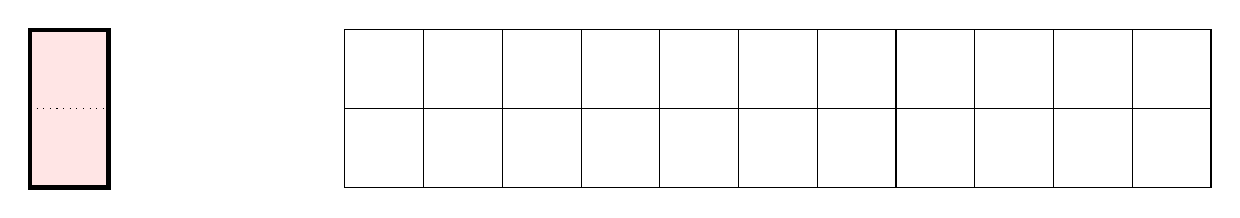
\begin{tikzpicture}[node distance=0.5cm]
      \filldraw[fill=red!10,ultra thick] (0,0) rectangle (1,2);
      \draw [dotted] (0,1) to (1,1);
      \draw (4,0) rectangle (15,2);
      \draw (4,1) to (15,1);
      \draw (5,0) to (5,2);
      \draw (6,0) to (6,2);
      \draw (7,0) to (7,2);
      \draw (8,0) to (8,2);
      \draw (9,0) to (9,2);
      \draw (10,0) to (10,2);
      \draw (11,0) to (11,2);
      \draw (12,0) to (12,2);
      \draw (13,0) to (13,2);
      \draw (14,0) to (14,2);
      \draw (15,0) to (15,2);
    \end{tikzpicture}
  \end{center}

  Your goal in this problem is to determine how many different ways there are to
  tile the checkerboard using your dominoes.

  To solve this problem, it is best to solve some smaller versions first. Let
  $S_n$ denote the number of different ways to tile a $2 \times n$ checkerboard.
  For example, $S_3 = 3$ as we see below:

  \begin{center}
    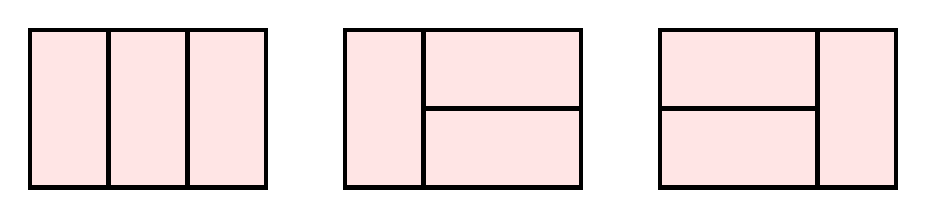
\begin{tikzpicture}[node distance=0.5cm]
      \filldraw[fill=red!10,ultra thick] (0,0) rectangle (1,2);
      \filldraw[fill=red!10,ultra thick] (1,0) rectangle (2,2);
      \filldraw[fill=red!10,ultra thick] (2,0) rectangle (3,2);
      \filldraw[fill=red!10,ultra thick] (4,0) rectangle (5,2);
      \filldraw[fill=red!10,ultra thick] (5,0) rectangle (7,1);
      \filldraw[fill=red!10,ultra thick] (5,1) rectangle (7,2);
      \filldraw[fill=red!10,ultra thick] (8,0) rectangle (10,1);
      \filldraw[fill=red!10,ultra thick] (8,1) rectangle (10,2);
      \filldraw[fill=red!10,ultra thick] (10,0) rectangle (11,2);
    \end{tikzpicture}
  \end{center}

  Make a table showing the values of $S_n$ for $1\leq n \leq 11$. As you are
  doing this, try to find a systematic way of finding all the tilings. Note any
  patterns that you find, and see if you can explain them. As a check, you
  should get $S_6=13$.
\end{problem}

\begin{probsolution}
\end{probsolution}

\newpage

\begin{problem}
  A certain puzzle has three pegs, the leftmost peg starting out with a tower of
  $n$ disks. The object of the puzzle is to move this tower to the rightmost
  peg. The rules are that you can only move one disk at a time, the disk has to
  be moved from one peg to another, and you can never place a larger disk on top
  of a smaller disk. The following picture shows the starting position of the
  puzzle when $n = 4$:

  \begin{center}
    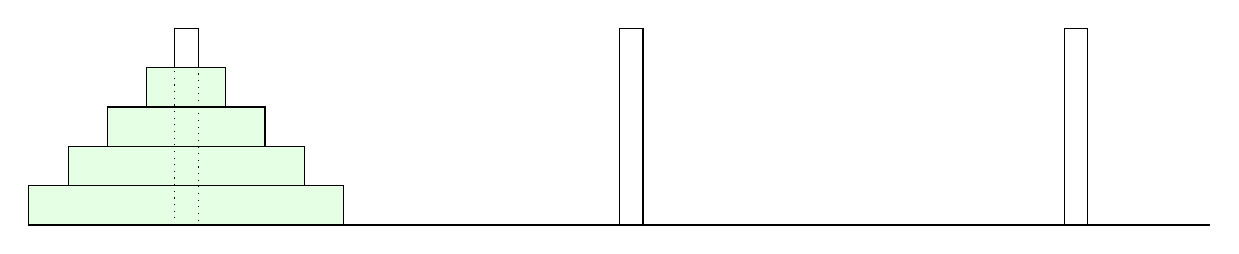
\begin{tikzpicture}[scale=0.5]
      \filldraw[fill=green!10]  (0,0) rectangle (8,1);
      \filldraw[fill=green!10]  (1,1) rectangle (7,2);
      \filldraw[fill=green!10]  (2,2) rectangle (6,3);
      \filldraw[fill=green!10]  (3,3) rectangle (5,4);
      \draw [dotted] (3.7,0) rectangle (4.3,5);
      \draw (3.7,4) rectangle (4.3,5);
      \draw (15,0) rectangle (15.6,5);
      \draw (26.3,0) rectangle (26.9,5);
      \draw [thick] (0,0) to (30,0);
    \end{tikzpicture}
  \end{center}

  Your goal in this problem is to determine the minimum number of moves needed
  to solve the puzzle when there are $11$ disks. Approach this in a similar way
  to what we did in problem \#13, by making a table showing the minimum number
  of moves to solve the $n$-disk game for $1 \leq n \leq 11$.
\end{problem}

\begin{probsolution}
\end{probsolution}
